\documentclass{article}
\usepackage[letterpaper]{geometry}
\geometry{verbose,tmargin=1in,bmargin=1in,lmargin=1in,rmargin=1in}

\usepackage[utf8]{inputenc}
\usepackage{amsmath}
\usepackage{listings}
\usepackage{graphicx}
\usepackage{enumitem}

\title{CIS 419/519: Homework 1}
\author{\{Yupeng Li\}}
\date{}

\begin{document}
    \maketitle
    Although the solutions are entirely my own, I consulted with the following people and sources while working on this homework:
     \{http://www.cs.utep.edu/vladik/cs5315.13/cs5315\_13kader.pdf\}
    
    \section{Decision Tree Learning}
        \begin{enumerate}[label=\alph*.]
            \item % a
            Show your work:
            \begin{equation*}
                \mathit{InfoGain}(\mathit{PainLocation}) = \mathit{Info(X)- Info(X | PainLocation)} 
            \end{equation*}
	    \[\mathit{Info(X) = -\frac{9}{14} \log_2 \frac{9}{14} - \frac{5}{14} \log_2 \frac{5}{14} = 0.9402}\]
	    \[\mathit{InfoGain(PainLocation) = Info(X) - \frac{5}{14} (-\frac{3}{5} \log_2 \frac{3}{5} - \frac{2}{5} \log_2 \frac{2}{5}) - \frac{5}{14} (-\frac{2}{5} \log_2 \frac{2}{5} - \frac{3}{5} \log_2 \frac{3}{5})-0 = 0.2467}\]
		
            \begin{equation*}
                \mathit{InfoGain}(\mathit{Temperature}) =\mathit{Info(X) - Info(X | Temperature)}
            \end{equation*}
            \[\mathit{= Info(X) - \frac{4}{14} (-\frac{2}{4} \log_2 \frac{2}{4} - \frac{2}{4} \log_2 \frac{2}{4}) - \frac{10}{14} (-\frac{7}{10} \log_2 \frac{7}{10} - \frac{3}{10} \log_2 \frac{3}{10}) = 0.02499}\] 
            
            
            \item % b
            Show your work:
            \[\mathit{SplitInformation(PainLocation) = -\frac{5}{14} \log_2 \frac{5}{14} -\frac{5}{14} \log_2 \frac{5}{14} - \frac{4}{14} \log_2 \frac{4}{14} = 1.5774}\]
            \begin{equation*}
                \mathit{GainRatio}(\mathit{PainLocation}) = \mathit{\frac{InfoGain(PainLocation)}{SplitInformation(PainLocation)}} = \mathit{\frac{0.2467}{1.5774}} = \mathit{0.156397}
            \end{equation*}
             \[\mathit{SplitInformation(Temperature) = -\frac{4}{14} \log_2 \frac{4}{14} -\frac{10}{14} \log_2 \frac{10}{14}  = 0.86312}\]
            \begin{equation*}
                \mathit{GainRatio}(\mathit{Temperature}) = \mathit{\frac{InfoGain(Temperature)}{SplitInformation(Temperature)}} = \mathit{\frac{0.02499}{0.86312}} = \mathit{0.028953}
            \end{equation*}
            
            \item % c 
            ~\\
            
            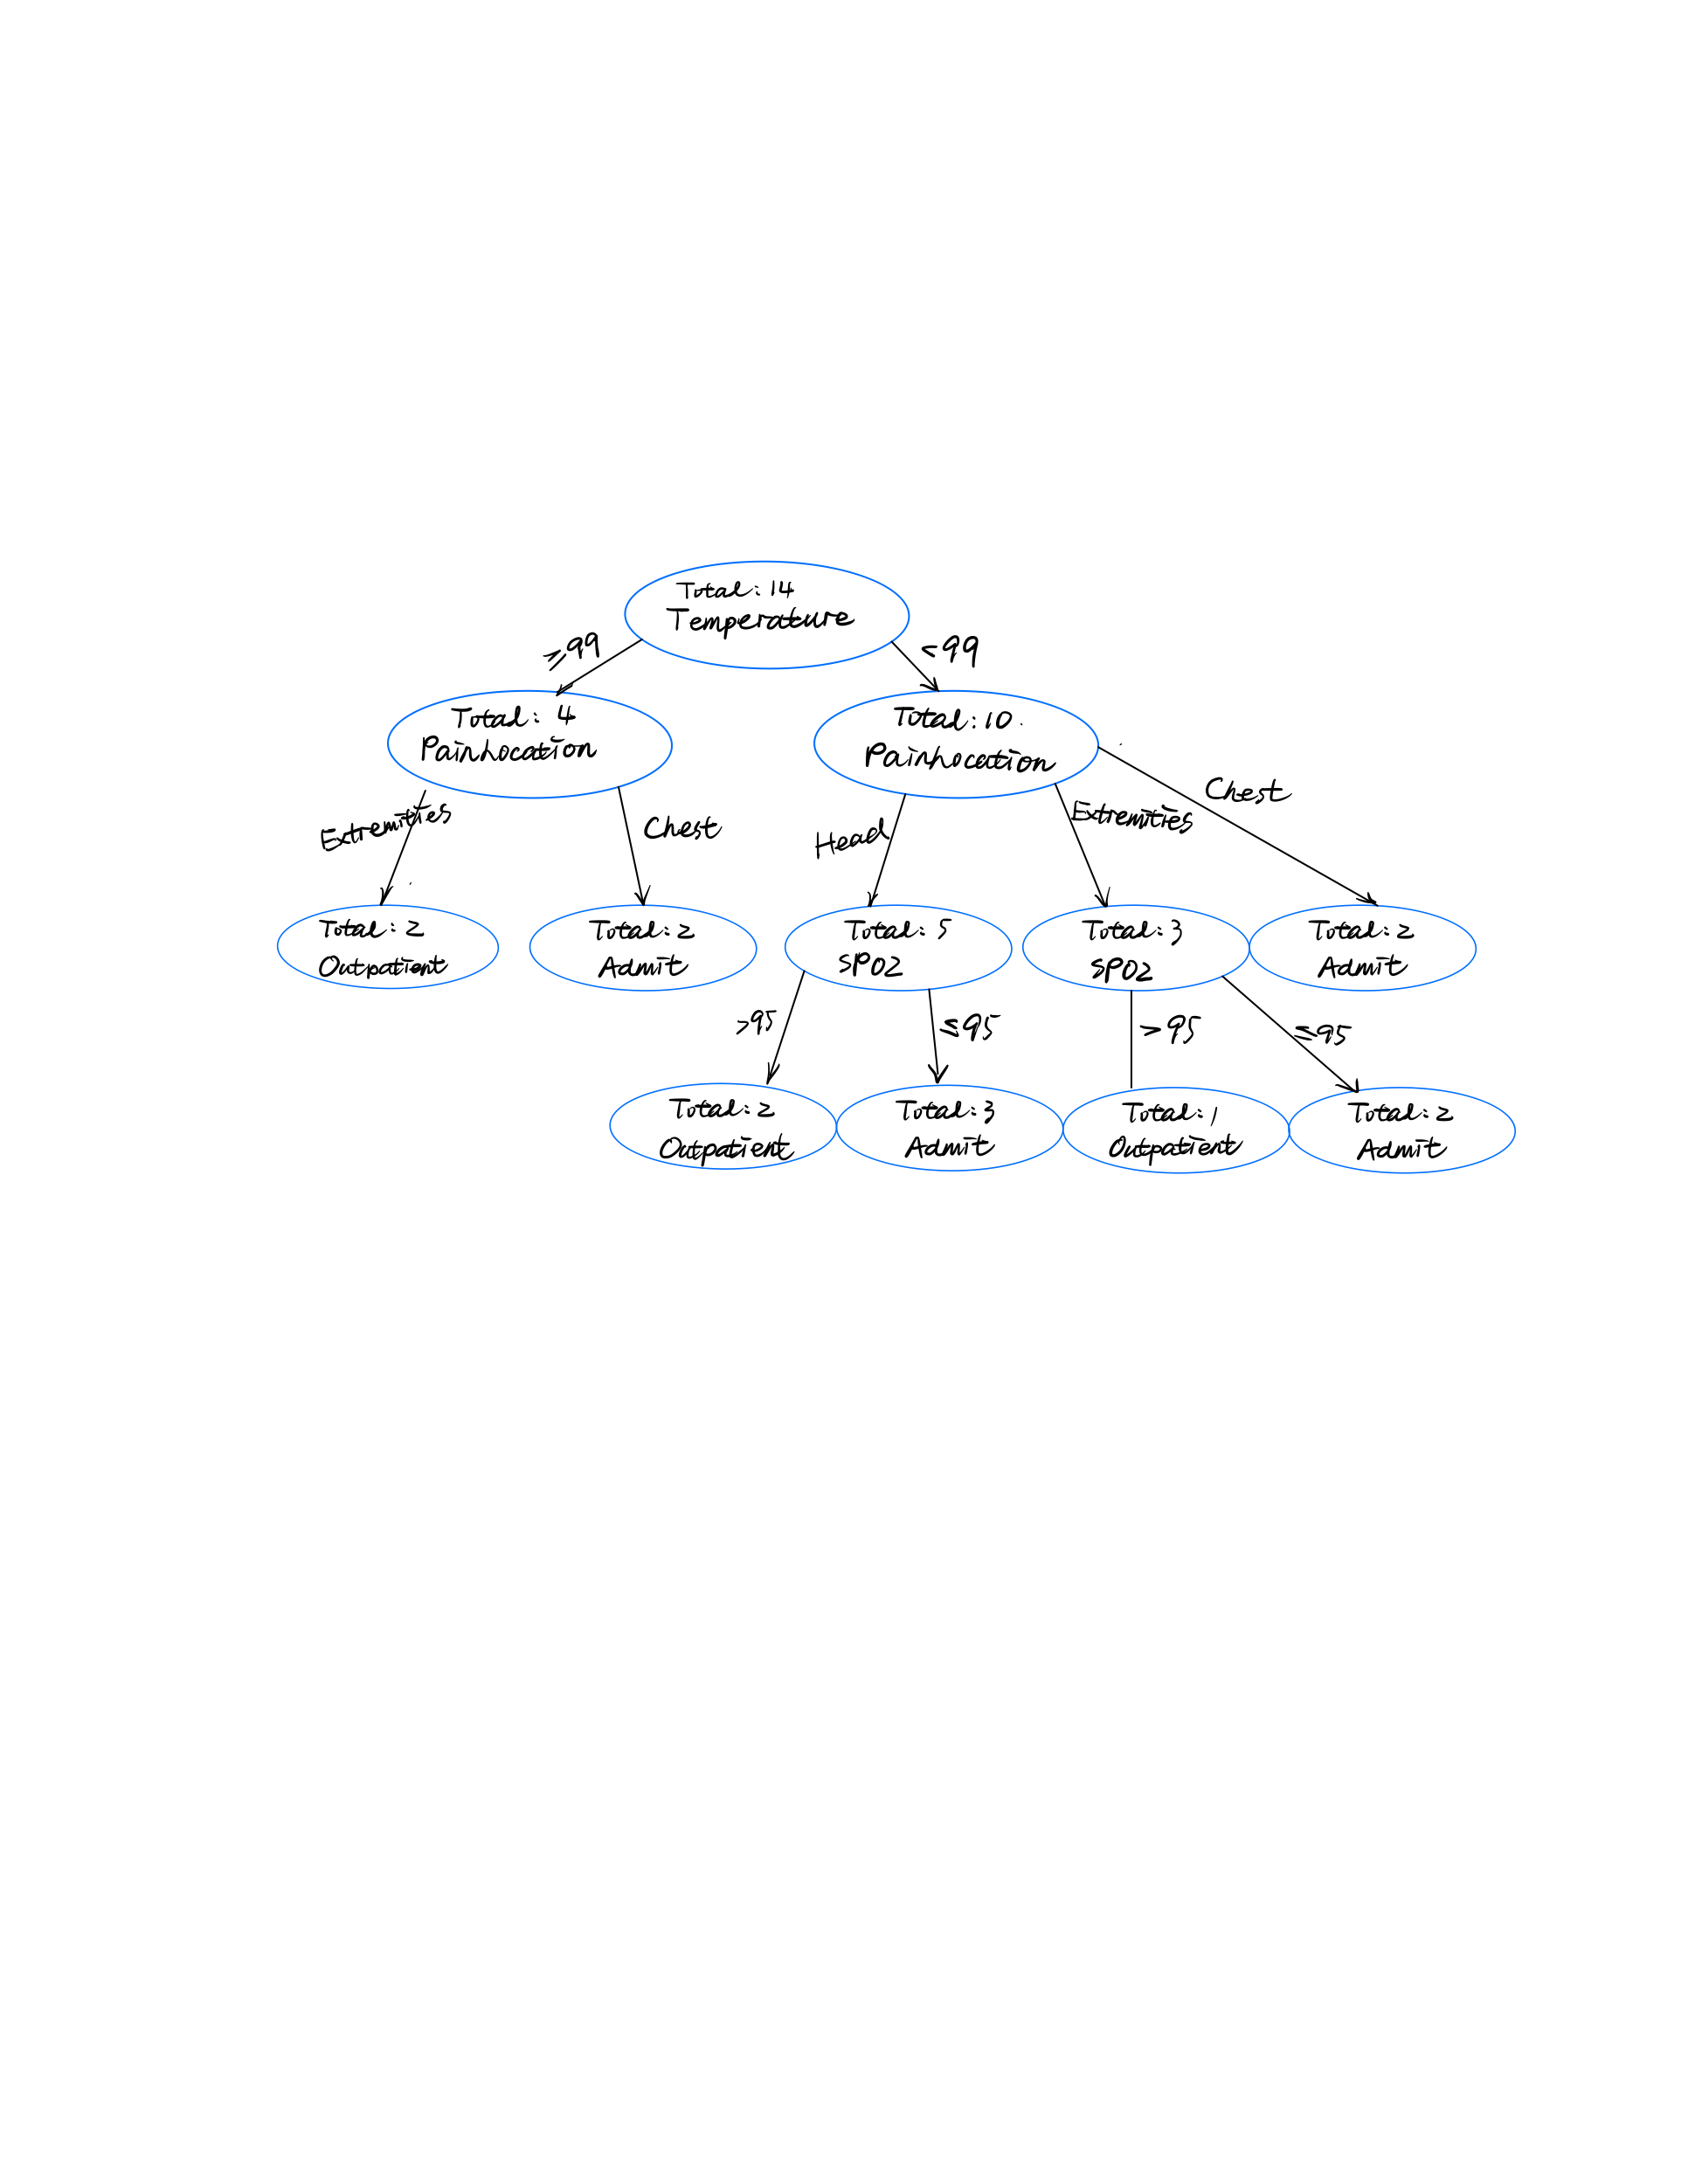
\includegraphics[width=0.8\textwidth]{HW1_Graph1}
                        
            \item % d
            No because finding the global optimal decision tree is NP hard  which has been proved in May, 1976. The advantage of ID3 is that it uses greedy approach which turns out to be really fast. ID3 will not produce the optimal decision tree, however, it gives good enough approximation. For more that 50\% of the datasets, ID3 can give the optimal solution.
        \end{enumerate}
        
       \section{Decision Trees \& Linear Discriminants [CIS 519 ONLY]}
        
        A decision tree can include oblique splits by taking linear combinations features when growing the decision tree. By doing it this way, our nodes would be classified using more than one feature, and this would result in oblique split in the decision tree which may not be parallel to the axes.
        
        For example, suppose we were training the data using the classic decision tree algorithms(ID3/C4.5), we are picking a single feature with highest information gain ratio for each node. If we want to do an oblique split, we pick the linear combination with highest information gain ratio for each node instead. The way we linearly combine those features is that we weigh each feature based on the information they can provide, then we multiply the features' information gain by their weight and sum up to get the info gain of this combination. After this, we choose the best combination of this node.
        
        
        \section{Programming Exercises}
        \textbf{Features}: What features did you choose and how did you preprocess them?
        
        I chose features from the original DataFrame using the function corrwith from Pandas library. It correlates the features from the dataframe to the predictions in y series. Then I rank them based on their absolute value and picked the top 30 of them.  Then I group them into groups of 10 and separate them into three different groups 1,2 and 3. (Before this step I already dropped 'SEQN' and 'DIQ010', since one of them is too correlated and the other is not at all related)
        
        After this, I start preprocessing the data. I first pick the desired features out from the original Dataframe. Then I drop features with more than 50\% missing rate while one-hot-encoding features whose datatypes are object instead of floats. Then I use the SimpleImputer from sklearn.impute to fill in the rest of NaNs with the mean of certain columns.
        
        For the first set, the features I chose are 'MCQ240K', 'LBDSGLSI', 'LBXSGL', 'LBXGLT', 'LBDGLTSI', 'CSQ120A', 'GTDCODE', 'DIQ070', 'DIQ050' which are the middle 10 of the top 30.
        
        For the second set, the features I chose are 'RHQ602U', 'RIDAGEYR', 'MCQ230C', 'OSQ120E', 'BMDAVSAD', 'BMXSAD2', 'BMXSAD1', 'BMXWAIST', 'DRD370JQ', which are the bottom 10 of top 30.
        
        For the third set, I am using the best I had from training the whole dataset which are 'LBDSGLSI', 'DIQ160', 'RIDAGEYR', 'DIQ180'.
        
        \noindent\textbf{Parameters}: What parameters did you use to train your best decision tree
        
        Criterion = 'entropy'  for tree growth and ccp\_alpha for pruning
        
        \noindent\textbf{Performance Table}: 
        \begin{center}
            \begin{tabular}{|c|c|c|}
                \hline
                Feature Set & Accuracy & Conf. Interval [519 ONLY]\\
                \hline
                DT 1 & 0.947 & [0.94166,0.9527]  \\
                DT 2 & 0.87699 & [0.867636,0.885344]  \\
                DT 3 & 0.9823 &  [0.97887,0.98586] \\
                \hline
        \end{tabular}
                \end{center}
        
        
        
        \textbf{Conclusion}: What can you conclude from your experience?
        
        From the tests above, we learn that we need to pick the most correlated features to get the best accuracies. However, we should also notice that not all best features are the best indications. Some features like DIQ010 which is "has a doctor ever told you that you have diabetes' have high correlation with diagnose classification. However, it doesn't even help when diagnosing a new patient. Besides, the reason why I am not picking the top10 from top 30 for decision tree is that it has too many NaNs in that. I think that is due to the nature of corrwith function itself. It is ranking columns with highest missing rate as 'Most correlated', that means we should probably drop the top 10 if we are picking our features using correlation.
\end{document}